\begin{center}

  \begin{tabular}{rp{16cm}lp{20cm}}%{rl}

  % after \\: \hline or \cline{col1-col2} \cline{col3-col4} ...

  论文地址:& \href{https://www.csie.ntu.edu.tw/~cjlin/papers/ffm.pdf}{https://www.csie.ntu.edu.tw/~cjlin/papers/ffm.pdf} \\
  来源:& RecSys, 2016 \\
  作者:& Yuchin Juan, Yong Zhuang, et al. \\

  源码:& \href{https://www.csie.ntu.edu.tw/~cjlin/libffm/}{libffm} \\

%  slides:& \href{http://yunshengb.com/wp-content/uploads/2017/03/nips_2018_r2l_workshop_talk.pdf}{{\footnotesize Convolutional Set Matching for Graph Similarity}}\\

  关键词:& \textbf{Machine learning, Click-through rate prediction, Computational advertising, Factorization machines} \\

  写于:& \date{2021-08-28}

  \end{tabular}

\end{center}

该论文\cite{juan2016field-aware}提出了FM模型的一个变种 --- FFM(Field-aware Factorization Machines)。FFM最初是应用的CTR预测任务上,模型与FM很类似。FFM也做了二阶特征交叉,交叉特征的权重的计算方式与FM略微不同。

\paragraph{问题定义}
解决CTR预测问题中特征稀疏、特征交叉的问题。

\paragraph{FFM}
FFM中将$n$个特征进行了分组,得到$f$个field,每个特征在每个field中都有一个$k$维的向量表示。对于交叉特征$x_{j_1}\cdot x_{j_2}$,其中$x_{j1}$属于field $f_1$,$x_{j_2}$同理,其权重计算方式为:$\boldsymbol{w}_{j_1, f_2} \cdot \boldsymbol{w}_{j_2, f_1}$,其中$\boldsymbol{w}_{j_1, f_2} \in \mathbb{R}^n$表示特征$x_{j_1}$在field $f_2$中的向量表示。

\begin{figure}[h]
	\centering
	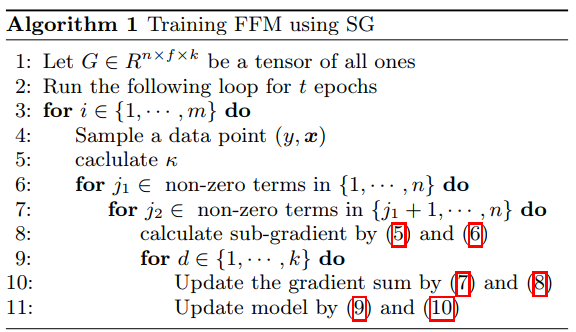
\includegraphics[width=.8\textwidth]{pics/ffm-sg.png}
	\caption{Training FFM with SGD}
	\label{fig:ffm-sg}
\end{figure}
使用SGD训练FFM的过程如Fig.\ref{fig:ffm-sg}所示,其中引用的公式$(5), (6), (7), (8), (9), (10)$分别是:
$$
\begin{aligned}
	&\boldsymbol{g}_{j_{1}, f_{2}} \equiv \nabla_{\boldsymbol{w}_{j_{1}, f_{2}}} f(\boldsymbol{w})=\lambda \cdot \boldsymbol{w}_{j_{1}, f_{2}}+\kappa \cdot \boldsymbol{w}_{j_{2}, f_{1}} x_{j_{1}} x_{j_{2}}\\
	&\boldsymbol{g}_{j_{2}, f_{1}} \equiv \nabla_{\boldsymbol{w}_{j_{2}, f_{1}}} f(\boldsymbol{w})=\lambda \cdot \boldsymbol{w}_{j_{2}, f_{1}}+\kappa \cdot \boldsymbol{w}_{j_{1}, f_{2}} x_{j_{1}} x_{j_{2}}
\end{aligned}
$$

$$
\begin{aligned}
	&\left(G_{j_{1}, f_{2}}\right)_{d} \leftarrow\left(G_{j_{1}, f_{2}}\right)_{d}+\left(g_{j_{1}, f_{2}}\right)_{d}^{2}\\
	&\left(G_{j_{2}, f_{1}}\right)_{d} \leftarrow\left(G_{j_{2}, f_{1}}\right)_{d}+\left(g_{j_{2}, f_{1}}\right)_{d}^{2}
\end{aligned}
$$

$$
\begin{aligned}
	&\left(w_{j_{1}, f_{2}}\right)_{d} \leftarrow\left(w_{j_{1}, f_{2}}\right)_{d}-\frac{\eta}{\sqrt{\left(G_{j_{1}, f_{2}}\right)_{d}}}\left(g_{j_{1}, f_{2}}\right)_{d}\\
	&\left(w_{j_{2}, f_{1}}\right)_{d} \leftarrow\left(w_{j_{2}, f_{1}}\right)_{d}-\frac{\eta}{\sqrt{\left(G_{j_{2}, f_{1}}\right)_{d}}}\left(g_{j_{2}, f_{1}}\right)_{d}
\end{aligned}
$$
Fig.\ref{fig:ffm-sg}中的$(5)$计算的是损失函数(包含了l2正则)关于$\boldsymbol{w}_{j_1, f_2}$的梯度,$(6)$同理。$(7)$则计算的是$(5)$中梯度的各个维度的平方和,$G$初始化为1,避免计算完后$G$太小导致$G^{-\frac{1}{2}}$太大,$(8)$同理。$(9)$则是对$\boldsymbol{w}_{j_1, f_2}$逐维度更新,其中$\eta$自定义的学习率,这就是实际更新交叉特征参数的步骤,$(7)$中计算的$G$相当于对梯度向量归一化(\tbc{red}{个人觉得论文上公式是不是写错了,$(7),(8)$中应该是$G_{j_1, f_2}$而不是$(G_{j_1,f_2})_d$}。

\paragraph{为什么要field-aware?}
FM相当于FFM的一个特例,只有1个field。与FM相比,FFM将特征分成多个fields,每个特征在每个field中都有一个向量表示(\tbc{red}{从这个角度看有点像解耦表征})。当一个特征$x_{j_1}$与其他特征组合时,FM只有一个向量用于计算,而FFM中,会根据另一个特征所属的field使用不同的向量进行计算,相当于对模型表达能力的一个细化,增强模型的表达能力。当然,FFM的参数量增加了,而且不可以像FM那样化简,因此其时间复杂度为$O(\bar{n}^2k)$,但FFM中隐向量的维度要远小于FM的维度。

\paragraph{Assign field to feature}
既然每个特征都属于一个field,那怎么划分呢?对于类别特征,很显然,一般都属于同一个field。对于数值特征,可以对其进行离散化后作为类别特征处理。还有一种就是单一特征的样本(只有一个特征),例如特征是文本的情况下,每个文本基本都是不一样的,如果都划分到一个field则退化成了FM,如果每个文本都是一个field则是很不实际的,因为一般样本的数量是很大的,对于这个问题论文中并没有进行给出方法,个人认为:将文本处理成向量,可以是bag of words,一些统计量、embedding等。

\paragraph{总结}

\begin{itemize}
	\item 将特征划分到fields,增强模型的表达能力,一个特征与不同field的特征交叉时使用不同的向量表示
	\item 能够应对较稀疏的数据,当数据不是很稀疏时,提升不是很明显
	\item 数值特征和单一特征划分field是个值得探讨的问题

\end{itemize}

